\section{CnC Ray Tracing Implementation}

% RRL: You're going to work on this...
Implementing ray tracing using CnC allows the algorithm to run on a
distributed system which is planned to be extensible to exascale
computers and reduces the need for expensive preprocessing seen with
many current systems. This is due to the dynamic nature of CnC
execution and is similar to the algorithm proposed by Navratil et al.
~\cite{navratil2014dynamic}. The CnC implementation beings by
partitioning data into voxels, this data is then distributed
dynamically at runtime.
%% RRL: Aren't partitioning and distibuting the same thing? You seem
%% to be saying that the data is partitioned both before and during
%% runtime.
The ray tracing portion of the algorithm is
iterative. Primary rays are sent into the system from the camera and
may give rise to secondary rays (shadow, reflection, refraction, etc.)
until all rays are fully traced.
%% RRL: Not clear what we mean by ``fully traced''.

Figure~\ref{fig:cnc} shows the proposed CnC graph for distributed ray
tracing.
%% RRL: What does the color coding mean?
It represents data collections as ovals and step collections
as rectangles, each with a name
(in upper case on its first line) and associated item tag(s) (in
square brackets on its subsequent lines). It also shows the
dependencies between them. The control collection for the proposed
model is static for all steps except TRACE\_VOXEL
and defined in an initialization step. The graph begins
execution when the object data, light data, and camera data are
provided, and terminates when the image is produced.
%% RRL: What if there are multiple frames?

\subsection{Tag Collections}

The tag collections are different for most data and step collections
%% RRL: Are these collections of ``item tags''
but share common elements. FRAME refers to one specific frame in the
case of an animation. INSTANCE refers to the current iteration.
%% RRL: What about this algorithm is iterative?
I, J, K are iterators over spatial data, or in the case of LIGHT, the
light index.
%% RRL: It's confusing to use ``I'' twice like this.

\subsection{Data Collections}

%% RRL: It would be more consistent to either drop the ``_DATA''
%% suffix or use it consistently.

OBJECT\_DATA contains input data for the scene from the environment.
In our case, it is in the form of a Wavefront ``\texttt{.obj}'' file.
DECOMPOSE\_DOMAIN splits this data into voxels and produces
VOXEL\_OBJECT\_DATA. Triangles that span multiple voxels are
duplicated. The LIGHT data collection contains data pertaining to any
light sources. VOXEL\_LIGHT\_DATA contains the same information as
LIGHT plus a traced light mesh for each wall of a voxel. CAMERA
contains the location and direction of the camera. RAY\_PACKET
contains all the rays that intersect a voxel wall for a given wall and
iteration. IMAGE contains the final image data.

\subsection{Step Collections}

\subsubsection{Decompose Domain}

DECOMPOSE\_DOMAIN takes the data to be traced as input and produces
subsets of that data based on voxel decomposition. As load balancing
is not a concern
% RRL: Have you adequately explained why not?
a fast uniformly spaced geometric distribution is sufficient. The
number of voxels produced is set at runtime and should be more than
the number of nodes available.

\subsubsection{Distribute Lights}

In order to reduce communication of secondary rays, DISTRIBUTE\_LIGHTS
lights is responsible for distributing light information to each
voxel. This guarantees each voxel will only need to communicate with
its direct neighbors. The light information produced for each voxel
contains the original light sources as well as a light source mesh for
each light and each wall of the voxel. The mesh is produced by tracing
rays from each light source to a uniform grid on a voxel wall. Where the
rays intersect the wall, a new directional light source is created to
light the cell. If the ray is blocked, the point light source will be
tagged as in shadow.

\begin{figure}[!htb]
\centering
\begin{subfigure}{.49\columnwidth}
 \centering
  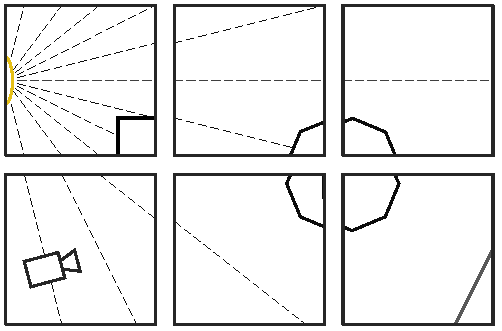
\includegraphics[width=.98\columnwidth]{drawings/Lights1.pdf}
  \caption{Initial light rays}
\end{subfigure}
\begin{subfigure}{.49\columnwidth}
 \centering
  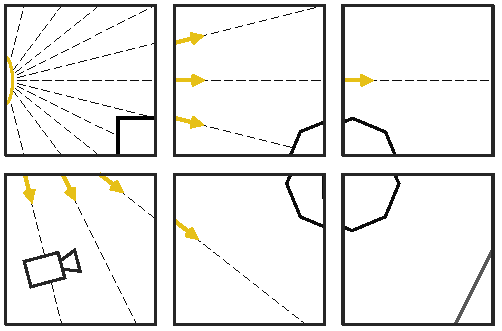
\includegraphics[width=.98\columnwidth]{drawings/Lights2.pdf}
  \caption{Point light sources}
\end{subfigure}
\caption{Light Ray Distribution}
\label{fig:light}
\end{figure}

\subsubsection{Distribute Rays}

DISTRIBUTE\_RAYS is responsible for sending each voxel its first iteration of ray information.  This is an empty set of data for all voxels except the voxel containing the camera if the camera is positioned within the domain.  If the camera is outside the domain, multiple voxels may receive data.

\subsubsection{Trace Voxel}

TRACE\_VOXEL is the heart of the application.  This step is iterative and prescribes the next iteration as long as there are rays still to trace and it has not reached a maximum threshold.  Trace voxel consumes ray packets from each of its neighbors.  It then traces the rays over its subset of the domain.  If a ray intersects with an object, secondary rays from each light source are considered if the corresponding point light source from the voxels light mesh is not in shadow.  Rays that reach the voxel walls are collected and passed to the corresponding neighbor on the next iteration.  As each CnC step instance will eventually be executed on a single node of a cluster the step code is integrating with Embree, Intel’s ray tracing kernel, in order to optimize per node performance.

\begin{figure}[!htb]
\centering
\begin{subfigure}{.49\columnwidth}
 \centering
  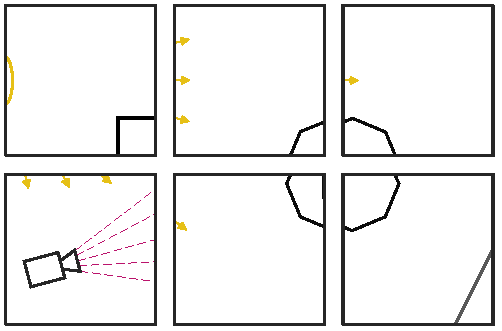
\includegraphics[width=.98\columnwidth]{drawings/Trace1.pdf}
  \caption{Distribute rays}
\end{subfigure}
\begin{subfigure}{.49\columnwidth}
 \centering
  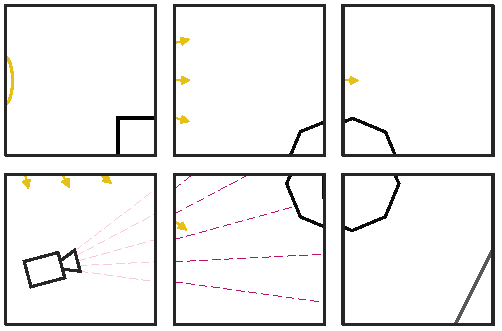
\includegraphics[width=.98\columnwidth]{drawings/Trace2.pdf}
  \caption{Trace voxel; iteration 1}
\end{subfigure}
\begin{subfigure}{.49\columnwidth}
 \centering
  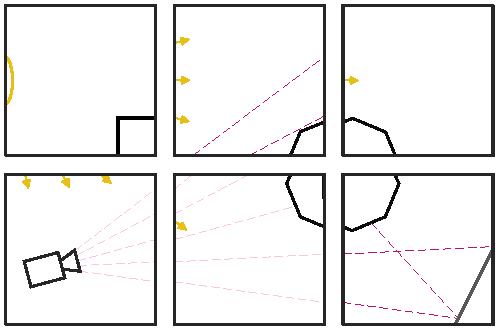
\includegraphics[width=.98\columnwidth]{drawings/Trace3.pdf}
  \caption{Trace voxel; iteration 2}
\end{subfigure}
\begin{subfigure}{.49\columnwidth}
 \centering
  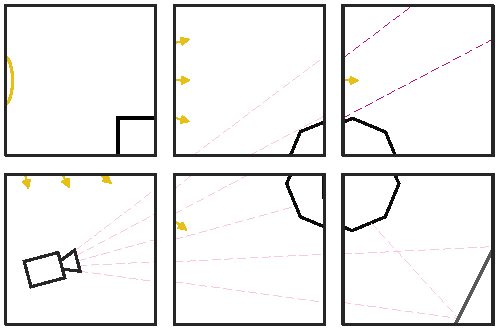
\includegraphics[width=.98\columnwidth]{drawings/Trace4.pdf}
  \caption{Trace voxel; iteration 3}
\end{subfigure}
\caption{Iterative Trace Voxel}
\label{fig:trace}
\end{figure}

\subsubsection{Produce Image}
When TRACE\_VOXEL has converged, a final set of ray packets will be
produced. Each ray in that packet contains the information necessary
to produce the final image; merging these is the responsibility of the
PRODUCE\_IMAGE step.

%%% Local Variables: 
%%% mode: latex
%%% TeX-master: "main"
%%% End: 
